\documentclass[12pt, twoside, a4paper]{article}
\usepackage[UTF8]{ctex}
\usepackage[left=0.6in, right=0.6in, top=0.7in, bottom=0.7in]{geometry}
\usepackage{fontspec}
\usepackage{xcolor}
\usepackage{tcolorbox}
\usepackage{listings}
\usepackage{hyperref}
\usepackage{graphicx}
\usepackage{subcaption}

\newfontface\mytt{FiraMono Nerd Font Mono}[Contextuals={WordInitial,WordFinal}]
% \newcommand{\inlinecode}[1]{\mytt #1}
\newcommand{\inlinecode}[1]{\setlength{\fboxsep}{0.8mm} \colorbox{lightgray!40}{\texttt{#1}}}

\begin{document}

\title{项目报告}
\author{王子睿、胡俞中、段林沛}
\date{\today}
\maketitle

\tableofcontents

\section{简介}

在项目根目录下输入 \inlinecode{make} 或者 \inlinecode{python src/main.py} 可以运行游戏。

本项目为SI100B课程的最终项目,
\href{https://github.com/o06660o/Kono-Aozora-ni-Yakusoku-o}{\textcolor{blue}{项目文件}}
已上传到了 GitHub。我们制作了一款类银河战士恶魔城游戏,玩家陷入梦境之中,手握一把丝线之剑,可在平台间跳跃与怪物搏斗。

战斗采用即时制,玩家通过键盘控制来进行移动和攻击,躲避怪物攻击的同时对其造成伤害。玩家击败怪物之后可以获得灵魂货币,
到商人NPC处可以用灵魂货币购买升级,击败怪物一定次数之后可以获得胜利。

程序的入口是 \inlinecode{main.py},其中的 \inlinecode{Game} 类负责游戏的整体逻辑。游戏的各个部分被分割到不同的模块。
\begin{itemize}
    \item \inlinecode{settings.py}:存储各种可调参数
    \item \inlinecode{level.py}:地图的控制
    \item \inlinecode{tile.py}: 地图中的障碍物
    \item \inlinecode{player.py}:玩家的控制
    \item \inlinecode{weapon.py}:玩家的三种武器
    \item \inlinecode{npc.py}:NPC 的控制
    \item \inlinecode{enemy.py}:敌人的控制
    \item \inlinecode{menu.py}:游戏的开始与结束画面
    \item \inlinecode{keys.py}:处理玩家输入
    \item \inlinecode{utils.py}:一些工具函数
    \item \inlinecode{debug.py}:一些调试用的函数
\end{itemize}


\section{项目内容}

\subsection{场景}

\subsubsection{大型场景}

游戏的场景是一个大型地图,地图中有两位 NPC 与会复活的敌人。

\begin{figure}[h!]
    \centering
    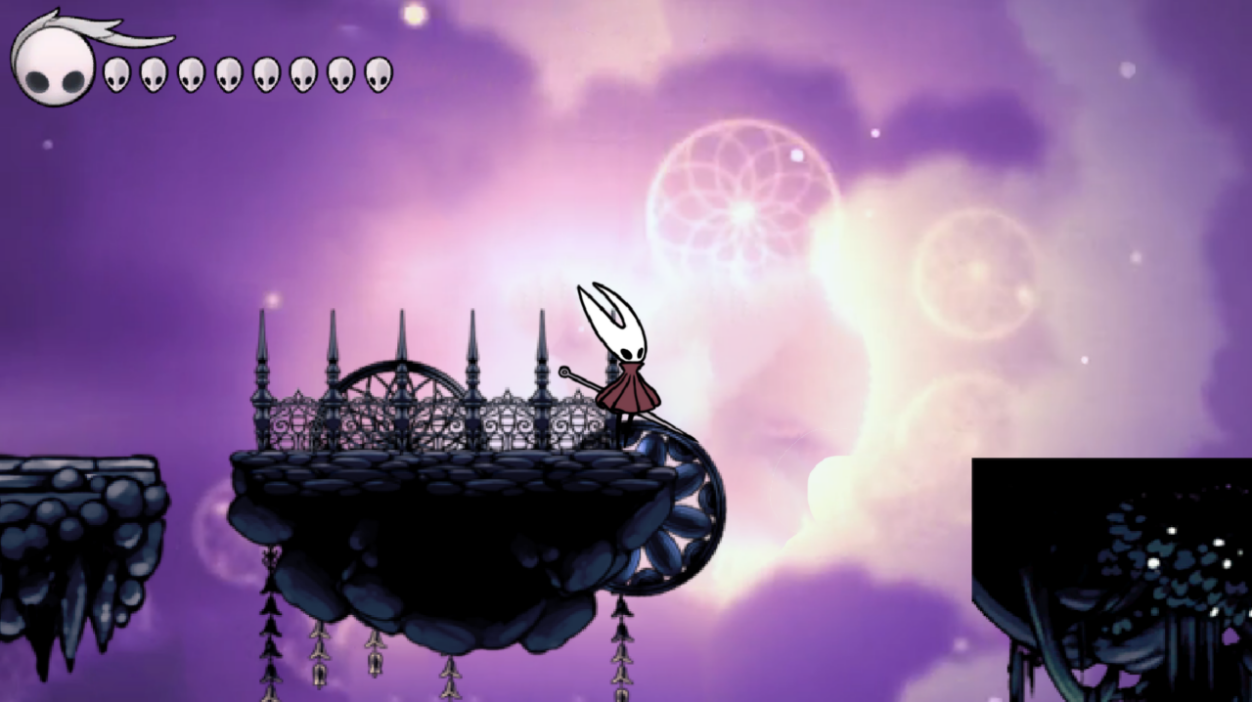
\includegraphics[width=0.7\textwidth]{assets/report/world.png}
    \caption{地图}
    % \label{fig3.1.1-0}
\end{figure}

整个地图由 \inlinecode{level\_dream.py} 中的 \inlinecode{LevelDream} 类控制,它继承自 \inlinecode{level.py}中定义的 \inlinecode{Level} 类。地图中的障碍物、敌人、角色与 NPC 都是在这里被创建实例,并在游戏循环中被更新。

游戏中的图像可能会重叠,为了让它们被正确显示我们定义了 \inlinecode{VisibleGroups} 类。先对可见图像按照 y 坐标排序,然后按照 "物品"、“敌人与NPC”、“主角” 的先后顺序绘制。

\subsubsection{交互对象}

地图中的障碍物在 \inlinecode{tile.py} 中定义。每个障碍物都有自己的碰撞箱,玩家与会与之发生碰撞。

\begin{figure}[h!]
    \centering
    \begin{subfigure}{0.45\textwidth}
        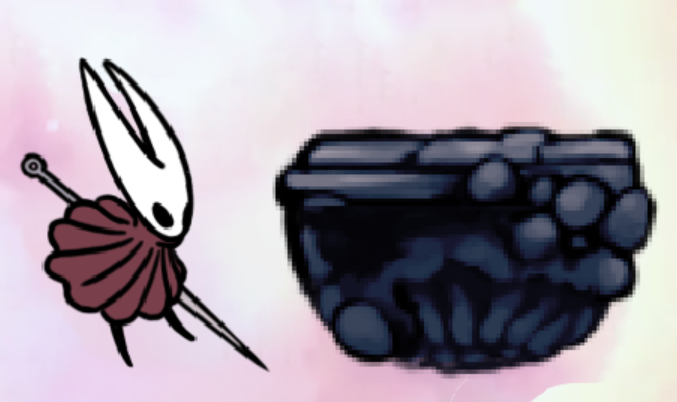
\includegraphics[width=\textwidth]{assets/report/tile0.png}
    \end{subfigure}
    \hspace{0.05\textwidth}
    \begin{subfigure}{0.45\textwidth}
        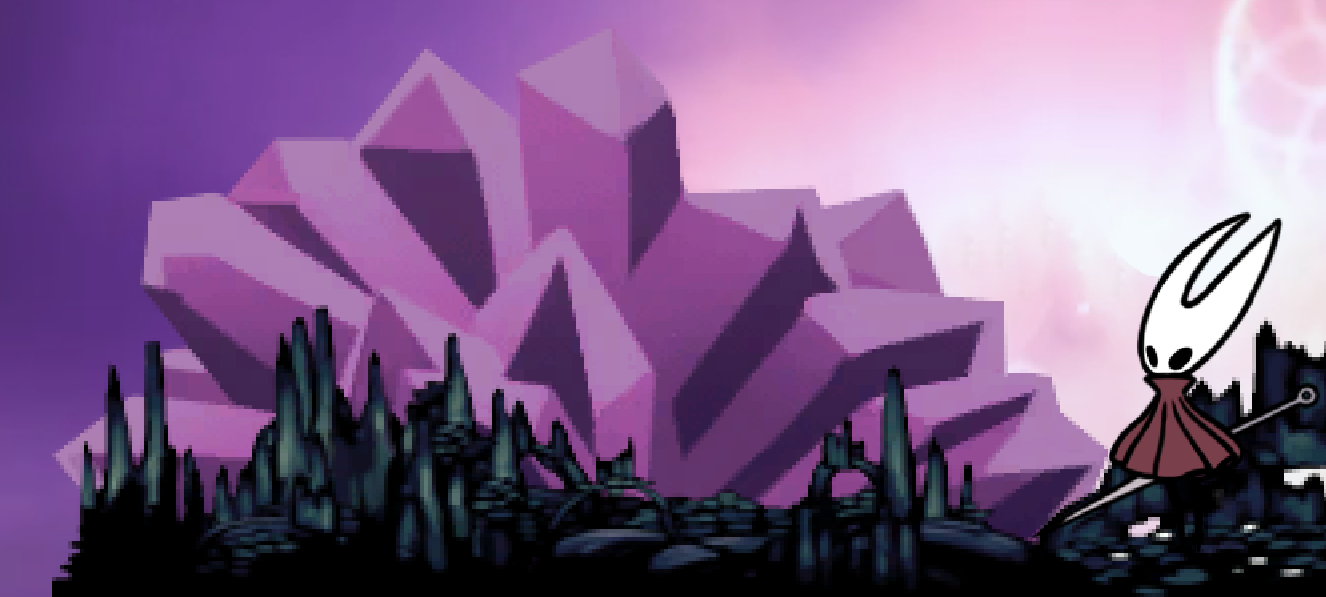
\includegraphics[width=\textwidth]{assets/report/tile1.png}
    \end{subfigure}
    \caption{地图中的障碍物}
\end{figure}

\subsection{角色}

\subsubsection{主角}

\paragraph{属性} 玩家拥有生命值与魔力值,被敌人打到会损失生命,释放魔法会消耗魔力。

\paragraph{移动} 玩家可以按下 <A> 和 <D> 来左右移动,按下 <Space> 跳跃,按下 <Shift> 冲刺,按住 <Shift> 疾跑。为了让玩家的移动更加自然,我们在玩家的跳跃过程中引入了重力加速度,并在检测到玩家落地的时候应用摩擦力。

\paragraph{攻击} 玩家可以按下 <J> 造成普通攻击,按下 <H> 丢出武器,进行远程攻击,按下 <U> 挥舞丝线,释放魔法。

\begin{figure}[h!]
    \centering
    \begin{subfigure}{0.4\textwidth}
        
\includegraphics[width=\textwidth]{assets/report/health0.png}
    \end{subfigure}
    \hspace{0.05\textwidth}
    \begin{subfigure}{0.4\textwidth}
        
\includegraphics[width=\textwidth]{assets/report/health1.png}
    \end{subfigure}
    \caption{玩家属性显示}
\end{figure}

\subsubsection{NPC}

游戏中有两位 NPC,一个是向导,另一个是铁匠,他们都继承自 \inlinecode{npc.py} 中定义的 \inlinecode{NPC} 类。
向导会在游戏开始时向玩家介绍游戏的基本操作,铁匠可以升级玩家的武器。

当玩家接近 NPC 的时候按下 <R> 可以开始对话,如果需要回复可以按下 </> 后输入内容,按下 <Enter> 发送。
玩家打开与铁匠的对话后按下 <B> 可以升级武器(消耗 10 单位货币)。

为了不漏掉玩家在输入对话的时候按下的每一个按键,我们在 \inlinecode{keys.py} 中通过处理游戏中获取到的每一个
\inlinecode{pygame.event.Event} 事件来管理输入。

具体的对话内容我们调用了 \inlinecode{python-openai} 库的 API,其中可能会有一些不可打印字符,我们在
\inlinecode{utils.py} 使用正则来 “标准化” 了一遍返回的字符串。

\begin{figure}[h!]
    \centering
    \begin{subfigure}{0.15\textwidth}
        
\includegraphics[width=\textwidth]{assets/report/tutorial.png}
        \caption{向导}
    \end{subfigure}
    \hspace{0.2\textwidth}
    \begin{subfigure}{0.4\textwidth}
        
\includegraphics[width=\textwidth]{assets/report/blacksmith.png}
        \caption{铁匠}
    \end{subfigure}
    \caption{NPC}
\end{figure}

\subsubsection{敌人}

地图中存在可以复活三次的敌人。敌人在每一帧都有一定概率转向,在距离初始位置太远时会强制转向。敌人每次被击败都会展示死亡动画,一段时间后复活。

初始时候玩家需要三次普通攻击才能杀死一个敌人,但是在升级两次之后就只需要一次攻击。每杀死一次敌人都会获得 5 单位货币。

\begin{figure}[h!]
    \centering
    \begin{subfigure}{0.4\textwidth}
        
\includegraphics[width=\textwidth]{assets/report/centipede_move0.png}
        \caption{移动}
    \end{subfigure}
    \hspace{0.05\textwidth}
    \begin{subfigure}{0.4\textwidth}
        
\includegraphics[width=\textwidth]{assets/report/centipede_death.png}
        \caption{死亡}
    \end{subfigure}
    \caption{敌人}
\end{figure}

\subsection{游戏机制}

\paragraph{核心机制} 玩家可以自由探索地图,与 NPC 对话,与敌人战斗。游戏的胜利条件是击败 \inlinecode{WIN\_COUNT} 次敌人。

\paragraph{碰撞系统} 游戏每一帧中玩家都会调用 \inlinecode{move()} 方法,其中会先进行 x 方向的移动,完成碰撞检测,再处理 y 方向的移动,最后第二次碰撞检测。每次碰撞检测玩家会与可碰撞精灵组的每一个元素进行碰撞检测。由于碰撞箱都是矩形,两两碰撞检测可以 O(1) 完成,在目前的数据规模下并不会造成卡顿。

\paragraph{资源系统} 玩家通过击败敌人获得灵魂货币,在铁匠处升级武器可以消耗货币。

\begin{figure}[h!]
    \centering
    
\includegraphics[width=0.08\textwidth]{assets/report/coin.png}
    \caption{货币}
\end{figure}

\subsection{游戏性}

\subsubsection{菜单}

菜单 UI 界面通过 photoshop 制作完成的花纹、游戏名、按键均由十分精美。点击 START 图标即可进入游玩,SETTING 图标可以通过按钮来调节音量,单击 QUIT 即可退出游戏。将鼠标置于三个按钮上会使按钮变粗并发出声音,其中涉及了碰撞的判断。此外,经过研究我们引入了 SPEECH RECOGNITION 功能,这使得玩家可以通过使用语音输入来控制菜单的一切功能,将会在 \textbf{语音识别系统} 部分详细说明。

\begin{figure}[h!]
    \centering
    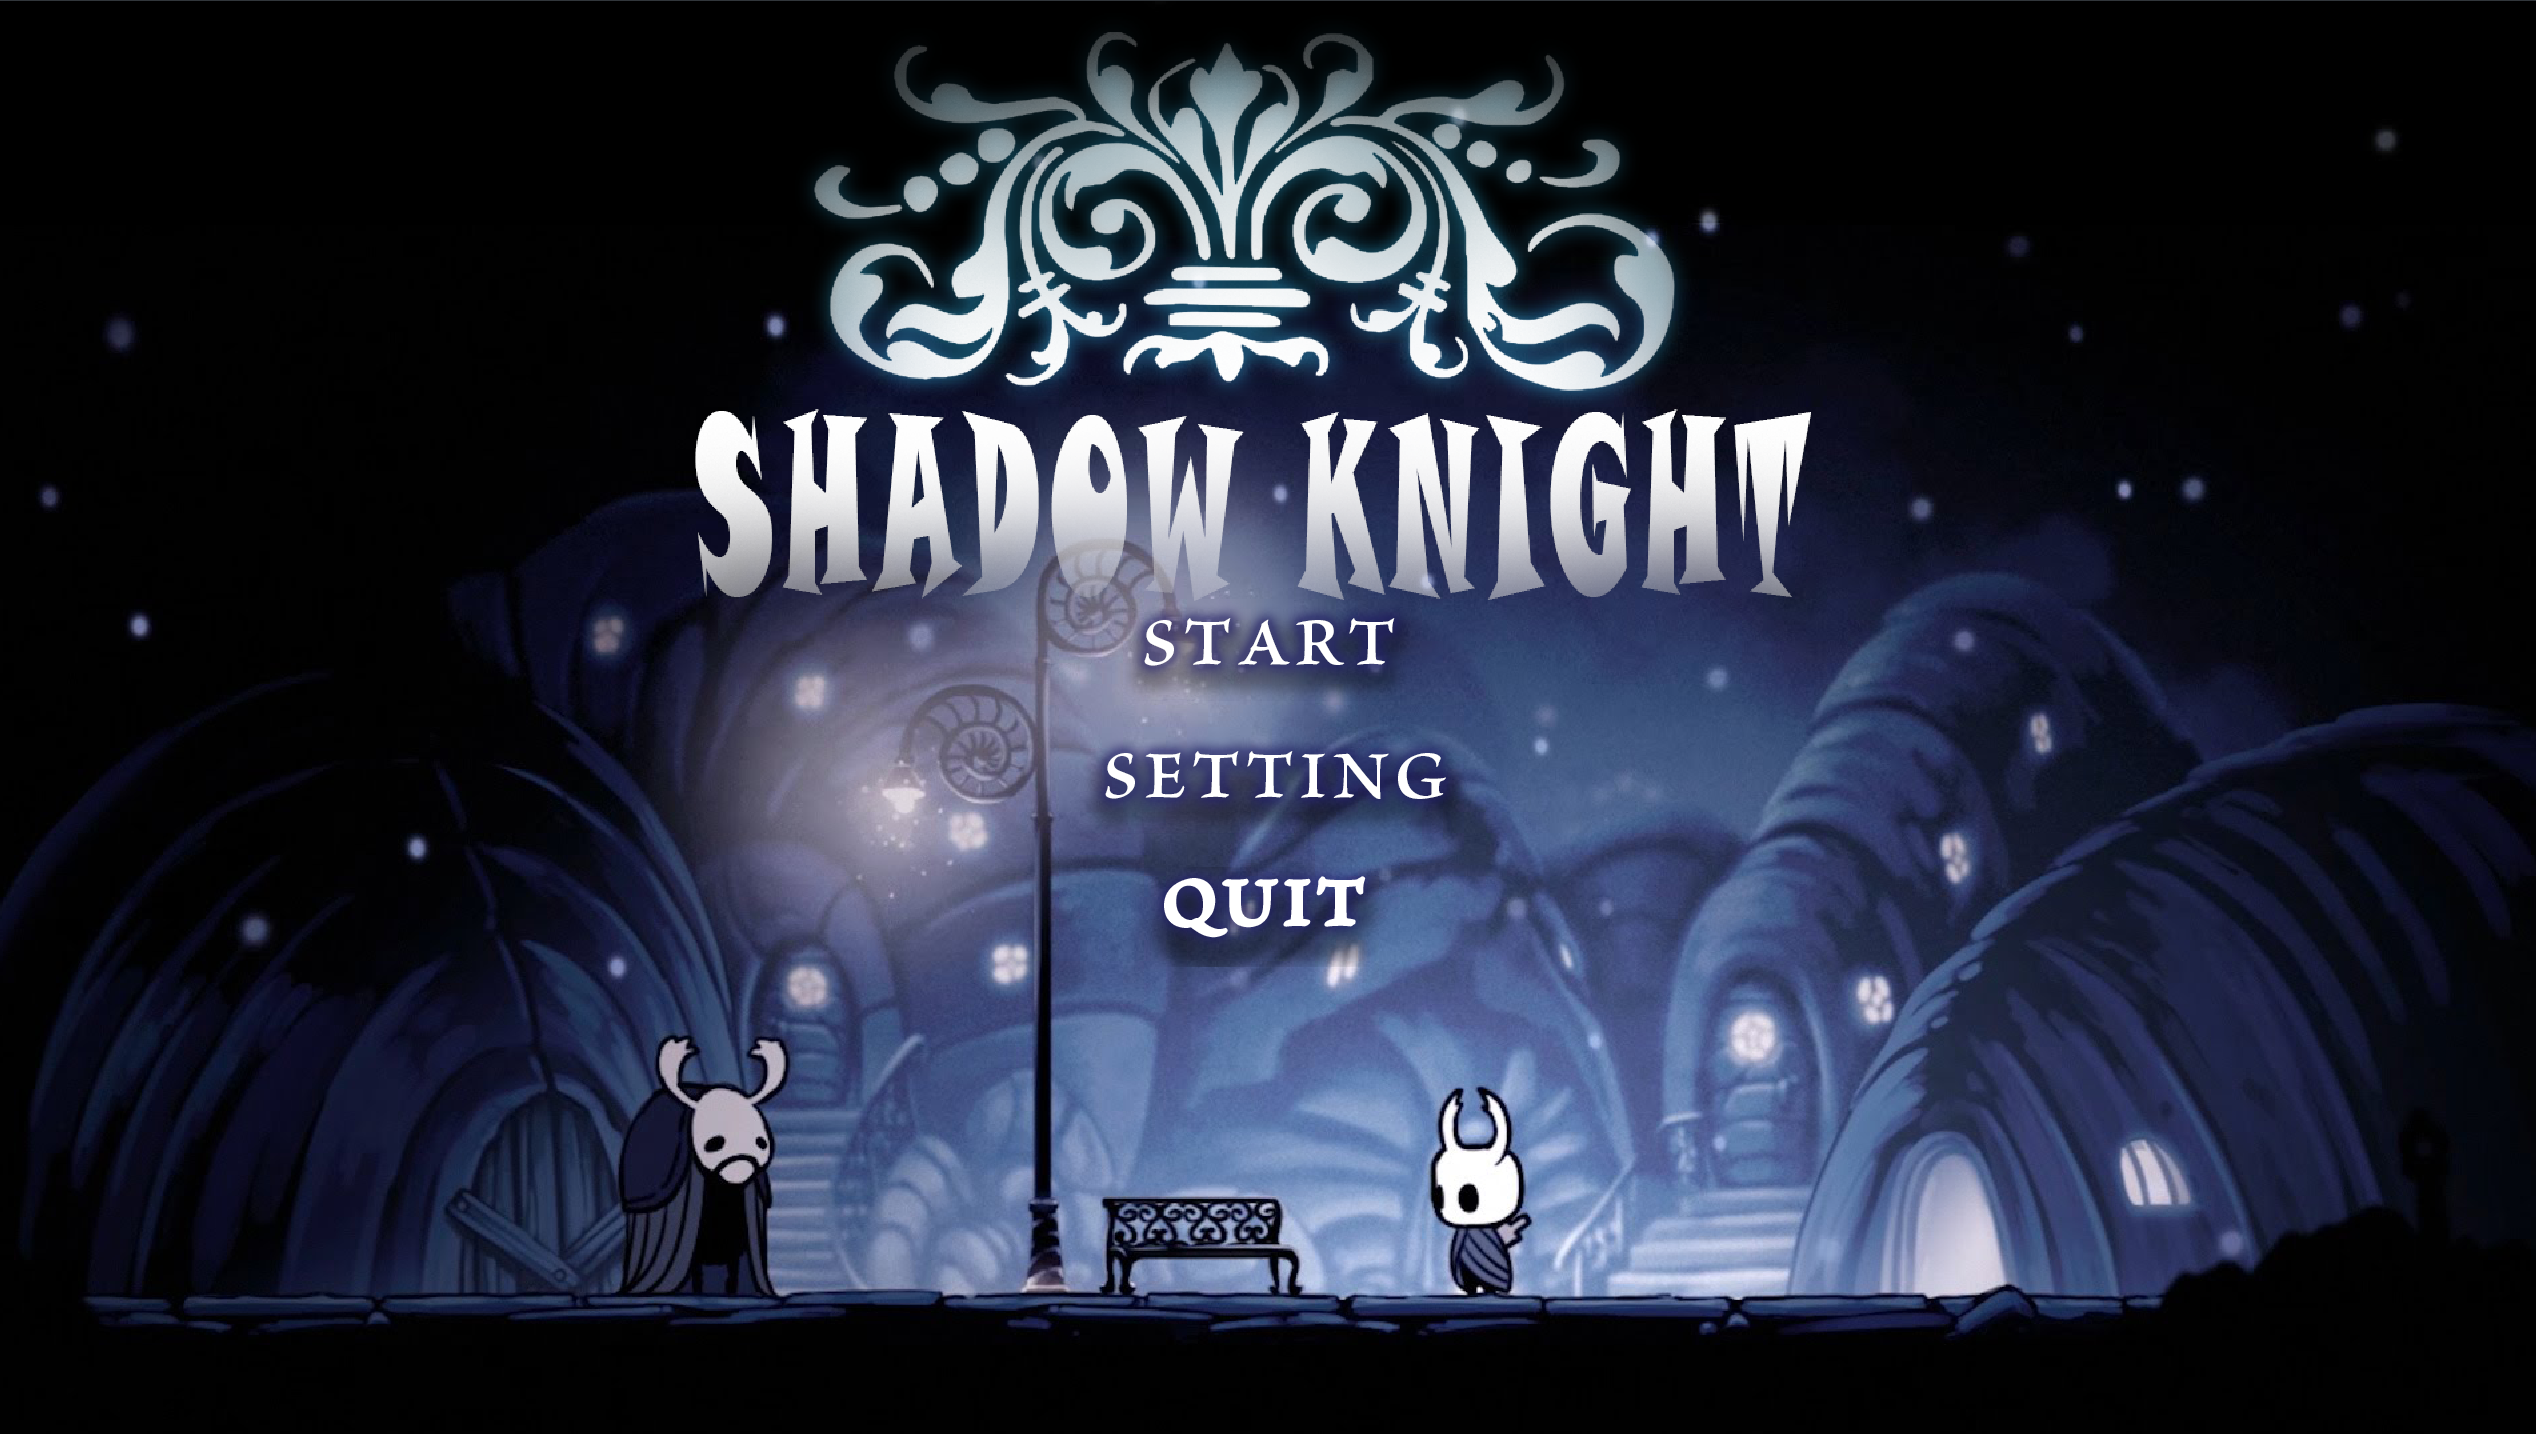
\includegraphics[width=0.7\textwidth]{assets/report/menu.png}
    \caption{菜单}
\end{figure}

\subsubsection{BGM}

游戏在开始菜单,游戏结束有不同的背景音乐。我们使用了 \inlinecode{pygame.mixer.music} 来播放音乐,可以通过菜单中的按钮来调节音量。

\section{创意}

\subsection{从零开始的游戏}

本项目没有使用助教提供的模板,整个代码的的框架都是自己设计实现的。虽然这可能给我们带来了一些不必要的麻烦,但是也让我们更加了解了整个游戏的实现细节。而且能够实现更不一样的游戏机制。

\subsection{调试模式}

本项目在开始的时候就为了调试设置了 \inlinecode{debug.py} 文件,其中的 \inlinecode{display()} 函数在有些时候能够比 \inlinecode{print()} 更优雅的显示变量的值,而的 \inlinecode{FreeCamera} 类可以代替玩家测试地图。另外本项目在运行的时候可以传入 \inlinecode{--DEBUG} 参数,开启调试模式并显示碰撞箱。

\subsection{语音识别系统}

在开始菜单界面其实是可以通过语音控制的。我们使用了 \inlinecode{python-speechrecognition} 库来调用 Google Speech API 来实现这个功能。玩家可以高呼 “开始”、“声音调大”、“声音调小”、“静音”、“退出” 来控制菜单。

\subsection{杂项}

\begin{itemize}
    \item 为了让玩家的移动更加自然,我们在玩家的跳跃过程中引入了重力加速度,并在检测到玩家落地的时候应用摩擦力。
    \item 为了让游戏在不同分辨率下自然显示,游戏中几乎每一个类都有 \inlinecode{scale} 参数。
\end{itemize}

\end{document}